\documentclass{beamer}

\usetheme{Boadilla}

\usepackage{amsmath}
\usepackage{amsfonts}
\usepackage{amsthm}
\usepackage{amssymb}
\usepackage{mathtools}
\usepackage{caption}
\usepackage{subcaption}
\usepackage{graphicx}
\usepackage{tikz}
\usepackage{hyperref}
\usepackage{pgfplots}
\usepackage{float}
\usepackage{url}
\usepackage{epigraph}

\hypersetup{colorlinks=true,allcolors=blue}

\renewcommand{\qedsymbol}{$\blacksquare$}

\newtheorem{fun}[]{Fun Fact}
\newtheorem{ques}[]{Main Question}
\newtheorem{prop}[theorem]{Proposition}
\newtheorem{cor}[theorem]{Corollary}
\setbeamertemplate{theorems}[ams style] 

\title{\textbf{Hackenbush \& Nim}}
\subtitle{Intro to Combinatorial Game Theory}
\date{\today}

\begin{document}
\begin{frame}
    \maketitle
\end{frame}


\begin{frame}{The Setting}
    %maybe add some pictures of the example games?
    \uncover<1->{
        A \emph{combinatorial game} is a two player game with
        \begin{enumerate}
            \item no hidden information
            \item and no chance elements
        \end{enumerate}
    }

    \uncover<2->{
        Examples: Tic-Tac-Toe, Chess, Checkers, Go
    }

    \uncover<3->{
        In all our games, we'll call our our two players \textbf{L}eft and \textbf{R}ight\\
    }

    \uncover<4->{
        \begin{ques}
            Given some state of our game, who wins under optimal play?
        \end{ques}
        CGT seeks to answer this questions with a mix of various algebraic and combinatorial techniques
    }
\end{frame}

\begin{frame}{Nim}
    \uncover<1->{
        \begin{center}
            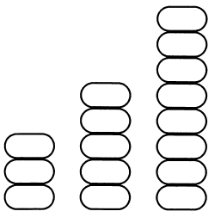
\includegraphics[scale=0.7]{nim-ex.png}
        \end{center}
    }

    \uncover<1->{
        Rules:
        \begin{itemize}
            \item<2-> There are several heaps of tokens
            \item<3-> Players \textbf{L} and \textbf{R} alternate taking turns
            \item<4-> During a turn, a player removes any number of tokens from \emph{one} heap
            \item<5-> First player unable to make a move loses
        \end{itemize}
    }
\end{frame}

\begin{frame}{Hackenbush}
    \uncover<1->{
        \begin{center}
            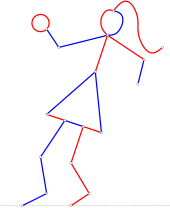
\includegraphics[scale=0.45]{hackenbush.png}
        \end{center}
    }

    \uncover<1->{
        Rules:
        \begin{itemize}
            \item<2-> There is an undirected graph
                \begin{itemize}
                    \item All edges are colored red or blue
                    \item There exists a vertex we denote \emph{ground}
                \end{itemize}
            \item<3-> Players b\textbf{L}ue and \textbf{R}ed alternate taking turns
            \item<4-> During a turn, a player deletes any edge of their color
                \begin{itemize}
                    \item Any edges no longer connected to \emph{ground} are also deleted
                \end{itemize}
            \item<5-> First player unable to make a move loses
        \end{itemize}
    }
\end{frame}

\begin{frame}{Domineering}
    \uncover<1->{
        \begin{center}
            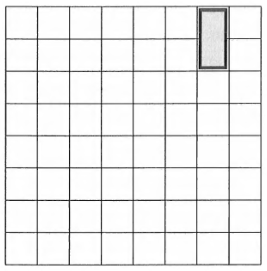
\includegraphics[scale=0.45]{domini.png}
        \end{center}
    }

    \uncover<1->{
        Rules:
        \begin{itemize}
            \item<2-> There is an $n \times n$ checkerboard
            \item<3-> Players L and R alternate taking turns
            \item<4-> During a turn, a player must place a $2 \times 2$ domino on the board
                \begin{itemize}
                    \item Each domino must cover exactly two squares
                    \item No two dominos can overlap
                    \item Left can only place dominos vertica\textbf{L}ly and Right can only place them ho\textbf{R}izontally
                \end{itemize}
            \item<5-> First player unable to make a move loses
        \end{itemize}
    }
\end{frame}

\begin{frame}{Vocab}
    \uncover<1->{
        \begin{definition}[Types of Play]
            \begin{itemize}
                \item[] \textbf{Normal Play} \; the player who makes the last move loses
                \item[] \textbf{Misere Play} \; the player who makes the last move wins
            \end{itemize}
        \end{definition} 
    }

    \uncover<2->{
        For all further discussion, we'll assume normal play
    }

    \uncover<3->{
        \begin{definition}
            \begin{itemize}
                \item[] \textbf{Partizan Games} \;  moves available to Left can be distinct from those available to Right
                \item[] \textbf{Impartial Games} \; both players have the same moves available at all times
            \end{itemize}
        \end{definition}
    }

    \uncover<4->{
        Examples: Hackenbush and Domineering are partizan where was Nim is impartial
    }

\end{frame}

\begin{frame}{Winning Nim Strategy}
    \begin{theorem}
        Let $G$ be a game of Nim with heaps $a_1, \ldots a_n$.
        \uncover<2->{
            Define $G$'s Nim value to be 
            $$a_1 \oplus a_2 \oplus \cdots \oplus a_n,$$
            where $\oplus$ is a bit-wise XOR.
        }

        \begin{enumerate}
            \item<3-> If $G$'s Nim value is zero, every move from $G$ leads to a game with non-zero Nim value
            \item<4-> If $G$'s Nim value isn't zero, there exists a move from $G$ to a game with zero Nim value
        \end{enumerate}
    \end{theorem}

    \uncover<5->{
        If $G$ has zero Nim value, the second player can always win. Why?
    }
\end{frame}

\begin{frame}{More Vocab}
    \uncover<1->{
        \begin{definition} 
            \begin{itemize}
                \item[] \textbf{game} \; an individual position in a combinatorial game 
                \item[] \textbf{ruleset}\; a system of playable rules
            \end{itemize}
        \end{definition} 
    }
    
    \uncover<2->{ 
        For instance, Hackenbush is a ruleset, not a game!
    }

    \uncover<3->{
        \begin{definition} 
            Let $G$ and $H$ be combinatorial games. 
            $H$ is a \textbf{left option} (resp. \textbf{right option}) of $G$ if Left (resp. Right) can move directly from $G$ to $H$
        \end{definition} 
    }

    \uncover<4->{
        \begin{definition} 
            Let $G$ and $H$ be combinatorial games. 
            $H$ is a \textbf{subposition} of $G$ if there exists a sequence of consecutive moves leading from $G$ to $H$
        \end{definition} 
    }
\end{frame}

\begin{frame}{Last Vocab Slide (I promise)}
    Let $G$ be a game.
    \begin{definition}
        \begin{enumerate}
            \item<2-> A \textbf{run} of $G$ of length $k$ is a sequence of positions
                $$G_0, G_1, G_2, \ldots, G_k$$
                such that $G_0 = G$ and $G_i$ is an option of $G_{i+1}$
                Note that $k$ can be $\infty$, in which case there is no last game $G_k$
            \item<3-> An \text{alternating run} is a run in which moves alternative between left and right: that is,
                $$G_{i+1} \text{ is a left option of } G_i \implies G_{i+2} \text{ is a right option of } G_{i+1}$$
            \item<4-> A \textbf{play} is alternating run that's infintely long or whose last game has no options for either player
        \end{enumerate}
    \end{definition}
\end{frame}

\begin{frame}{Outcome Classes}
    \uncover<1->{
        \begin{theorem}[Fundamental Theorem of Short Games]
            Let $G$ be a short game and assume normal play.
            \begin{enumerate}
                \item Either Left can force a win by playing first on $G$ or else Right can force a win playing second
                \item Either Right can force a win by playing first on $G$ or else Left can force a win playing second
            \end{enumerate}
        \end{theorem}
    }

    \uncover<2->{
        Every short game therefore belongs to one of the four outcome classes
        \begin{itemize}
            \item[$\mathcal N$] first player (the \textbf{N}ext player) can force a win
            \item[$\mathcal P$] second player (the \textbf{P}revious player) can force a win
            \item[$\mathcal L$] Left can force a win, no matter who moves first
            \item[$\mathcal R$] Right can force a win, no matter who moves first
        \end{itemize}
    }
\end{frame}

\begin{frame}{Adding Two Games}
    %include a picture of two games next to each other; Nim and Hackenbush
    \begin{definition}
       Given two games $G$ and $H$, the games $G+H$ is as follows:
       \begin{enumerate}
            \item<2-> Games $G$ and $H$ are placed side by side
            \item<3-> A player must move in exactly one of $G$ or $H$ (not both!)
       \end{enumerate}
    \end{definition}
\end{frame}

\begin{frame}{Fundamental Equivalence}
    %include the nontrivial 
    \uncover<2->{
        \begin{center}
            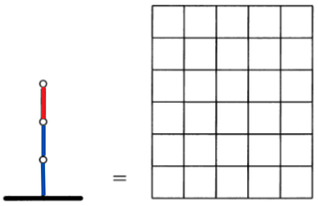
\includegraphics[scale=0.7]{hacken-domin.png}
        \end{center}
    }
    \begin{definition}
        For short games $G$ and $H$, we write $G = H$ if  
        $$o(G+X) = o(H+X) \text{ for all short games } X$$
    \end{definition}
\end{frame}

\begin{frame}{Where to Learn More!}
    Thank you for playing and listening!
    \vspace{10mm}
    
    
    Further reading:
    \begin{itemize}
        \item This great Hackenbush videogame.
            \begin{itemize}
                \item itch.io link: \href{https://fi-le.itch.io/hackenbush}{https://fi-le.itch.io/hackenbush}
                \item Github: \href{https://github.com/lennart-finke/hackenbush}{https://github.com/lennart-finke/hackenbush}
            \end{itemize}
        \item This Youtube video about Hackenbush. 
            \begin{itemize}
                \item \href{https://www.youtube.com/watch?v=ZYj4NkeGPdM}{HACKENBUSH: a window to a new world of math}
                \item One of the best math-tube videos ever IMO!
            \end{itemize}
        \item The CGT Bible: Winning Ways for your Mathematical Plays
    \end{itemize}
\end{frame}

\end{document}
